\documentclass[11pt, solution, letterpaper]{format}
\usepackage[utf8]{inputenc}
\setlength{\parindent}{0 in}

\usepackage{tikz}
\usetikzlibrary{arrows,automata}
\usepackage{amsmath}
\usepackage{graphicx}
\graphicspath{ {./images/} }
\usepackage[utf8]{inputenc}
\usepackage{enumerate}
\usepackage{amsmath,amssymb,amsthm}
\usepackage{listings}
\renewcommand{\qedsymbol}{$\blacksquare$}
\setlength\parindent{0pt}
\usepackage{tikz}
\usepackage{pgf}
\usepackage{tikz}
\usetikzlibrary{arrows,automata}
\usepackage{hyperref}
\newcommand{\noin}{\noindent}
\usepackage{enumerate}
\usepackage{tikz}
\usepackage{pgf}
\usepackage{tikz}
\usepackage{hyperref}
% \usepackage{booktabs}
\usepackage{cancel}

% \pagestyle{empty}

\setlength{\oddsidemargin}{-0.25 in}
\setlength{\evensidemargin}{-0.25 in}
\setlength{\topmargin}{-0.9 in}
\setlength{\textwidth}{7.0 in}
\setlength{\textheight}{9.0 in}
\setlength{\headsep}{0.75 in}
\setlength{\parindent}{0 in}
% \setlength{\parskip}{-.10 in}
\usepackage{epsf}
\usepackage{pseudocode}
% \usepackage{times}
% \usepackage{mathptm}

\def\O{\mathop{\smash{O}}\nolimits}
\def\o{\mathop{\smash{o}}\nolimits}
\newcommand{\e}{{\rm e}}
\newcommand{\R}{{\bf R}}
\newcommand{\Z}{{\bf Z}}
\newcommand\tab[1][1cm]{\hspace*{#1}}




\begin{document}
Problem Set 6\\
Julia Pearl\\

I collaborated with Rodrigo Daboin Sanchez. All code and problems were done independently.
\clearpage
\section{Recurrence}
We have considered a random walk with a completely reflecting boundary at 0– that is, whenever position 0
is reached, with probability 1 we move to position 1 at the next turn. Consider now a random walk with a
partially reflecting boundary at 0– whenever position 0 is reached, with probability 1/2 we move to position 1
at the next turn, and with probability 1/2 we stay at 0. Everywhere else the random walk either moves up or
down 1, each with probability 1/2.
Find the expected number of moves to reach n starting from position i using a random walk with a partially
reflecting boundary. (You may assume there is a unique solution to this problem, as a function of n and i; you
should prove that your solution satisfies the appropriate recurrence.)

In this problem, we know that:\\
$$E(n) = 0 $$ because when position is n, then the expected value of steps to n is equal to 0.\\
We also know that:
$$E(i) = \frac{E(i + 1)}{2} + \frac{E(i - 1)}{2} + 1 \text{ for } 0 < i < n$$
because the probability that the position goes closer or farther from n is 1/2 and the step in one of those directions adds 1 to the expected value. This was given to us in lecture.\\
Something that is unique to this problem is the following:
$$E(O) = \frac{E(0)}{2} + \frac{E(1)}{2} + 1 $$
Instead of E(0) being equal to E(1) + 1, there is a 50 percent probability that the position will remain at 0.

Again, this is what differentiates this problem from the lecture's problem. However, just as we solved the lecture problem's recurrence relation using that E(0) case, we can do that here as well:
$$E(O) = \frac{E(0)}{2} + \frac{E(1)}{2} + 1 $$
$$\frac{E(0)}{2} = \frac{E(1)}{2} + 1 $$
$$E(O) = E(1) + 2 $$
$$E(O) - 2 = E(1) $$
$$E(1) = E(O) - 2 = E(0) - 1*(1 + 1)$$

We can substitute this result into the recurrence for E(1) to get an expression for E(2) in terms of E(0):
$$E(1) = \frac{E(2)}{2} + \frac{E(0)}{2} + 1 = E(O) - 2$$
$$\frac{E(2)}{2} + \frac{E(0)}{2} + 1 = E(O) - 2$$
$$\frac{E(2)}{2} = \frac{E(0)}{2} - 3$$
$$E(2) = E(0) - 6 = E(0) - 2(2 + 1)$$

We can then substitute the results for E(2) and E(1) into the recurrence for E(2) to get an expression for E(3) in terms of E(0). 
$$E(2) = \frac{E(3)}{2} + \frac{E(1)}{2} + 1 = E(0) - 6 $$
$$E(2) = \frac{E(3)}{2} + \frac{E(0) - 2}{2} + 1 = E(0) - 6 $$
$$\frac{E(3)}{2} + \frac{E(0)}{2} = E(0) - 6 $$
$$\frac{E(3)}{2} = \frac{E(0)}{2} - 6 $$
$$E(3) = E(0) - 12 = E(0) - 3(3 + 1)$$

We can see a pattern that has maintained for E(0), E(1), E(2), and E(3): $$E(i) = E(0) - i(i + 1)$$. To confirm this, we will get calculate the results for E(4): 
$$E(3) = \frac{E(4)}{2} + \frac{E(2)}{2} + 1 = E(0) - 12 $$
$$E(2) = \frac{E(4)}{2} + \frac{E(0) - 6}{2} + 1 = E(0) - 12 $$
$$\frac{E(4)}{2} + \frac{E(0)}{2} - 2 = E(0) - 12 $$
$$\frac{E(4)}{2} = \frac{E(0)}{2} - 10 $$
$$E(4) = E(0) - 20 = E(0) - 4(4 + 1)$$

The pattern of E(i)= E(0) - i*(i + 1) holds. Now, we can find the correct value for E(0) in terms of n by plugging in n for i (we are incorporating our base case of E(n) = 0):
$$ E(n) = E(0) - n(n + 1)$$
$$ 0 = E(0) - n(n + 1)$$
$$ E(0) = n(n + 1)$$

We now have an equation for the expected number of moves to reach n from any position i (in which i is in the range [0, n]):
$$E(i) = n(n + 1) - i(i + 1)$$

\clearpage
\section{Max Flow}
Find the maximum flow from s to t and the minimum cut between s and t in the network below, using the
method of augmenting paths discussed in class. (This means give the flow along each edge, along with the
final flow value; similarly, give the edges that cross the cut, along with the final cut value.) Show the residual
network at the intermediate steps as you build the flow. (If you need more information on the algorithm, it’s
called the Ford-Fulkerson algorithm.)\\

\begin{tikzpicture}[->,>=stealth',shorten >=1pt,auto,node distance=4cm,
                    semithick]
  \tikzstyle{every state}=[fill=black, anchor=center, draw=none,text=white]
  \tikzstyle{lab}=[fill=white, anchor=center, text=black]
  \tikzstyle{quiz}=[fill=white, anchor=center, text=red]

  \node[state] (S)                    {$s$};
  \node[state] (A) [above right of=S] {$a$};
  \node[state] (B) [right of=A]       {$b$};
  \node[state] (C) [below right of=S] {$c$};
  \node[state] (E) [below right of=A] {$e$};
  \node[state] (D) [right of=C]       {$d$};
  \node[state] (T) [right of=E]       {$t$};

  \path (S) edge              node[lab] {4} (A)
            edge              node[lab] {5} (C)
        (A) edge              node[lab] {3} (B)
            edge              node[lab] {1} (E)
            edge              node[lab] {2} (D)
        (B) edge              node[lab] {4} (T)
        (C) edge              node[lab] {1} (E)
            edge              node[lab] {3} (D)
            edge              node[lab] {1} (A)
        (D) edge              node[lab] {3} (T)
        (E) edge              node[lab] {2} (T);
\end{tikzpicture}\\

We can perform Ford-Fulkerson using a depth first search. We will refer to edges in the direction of the flow as $f$ edges. We will refer to edges in the opposite direction of flow as $r$ edges. We explore every path and send as many units as the bottleneck of each path will allow (that will fulfill requirements of $f$ and $r$ edges). We will display, on each $f$ edge, the path's capacity minus its flow. We will display on each $r$ edge, the path's capacity minus its residual network. We will not be able to add more to a particular path when one of the $f$ edges holds a value of 0 or the value of one of the $r$ edges in the path is equal to 0. (going forwards is full or going backwards is empty). \\

Before we begin, let's add the $r$ edges to our graph and set the flow of each $f$ edge to capacity:\\

\begin{tikzpicture}[->,>=stealth',shorten >=1pt,auto,node distance=4cm,
                    semithick]
  \tikzstyle{every state}=[fill=black, anchor=center, draw=none,text=white]
  \tikzstyle{lab}=[fill=white, anchor=center, text=black]
  

  \node[state] (S)                    {$s$};
  \node[state] (A) [above right of=S] {$a$};
  \node[state] (B) [right of=A]       {$b$};
  \node[state] (C) [below right of=S] {$c$};
  \node[state] (E) [below right of=A] {$e$};
  \node[state] (D) [right of=C]       {$d$};
  \node[state] (T) [right of=E]       {$t$};

  \path (S) edge              node[lab] {4} (A)
            edge              node[lab] {5} (C)
        (A) edge              node[lab] {3} (B)
            edge              node[lab] {1} (E)
            edge              node[lab] {2} (D)
        (B) edge              node[lab] {4} (T)
        (C) edge              node[lab] {1} (E)
            edge              node[lab] {3} (D)
            edge              node[lab] {1} (A)
        (D) edge              node[lab] {3} (T)
        (E) edge              node[lab] {2} (T);
        
   \path (A) [->,bend left=15]  edge[dashed] node {0} (S)
             [->,bend left=15]  edge[dashed] node {0} (C)
         (B) [->,bend left=15]  edge[dashed] node {0} (A)
         (C) [->,bend left=15]  edge[dashed] node {0} (S)
         (D) [->,bend left=15]  edge[dashed] node {0} (C)
             [->,bend left=15]  edge[dashed] node {0} (A)
         (E) [->,bend left=15]  edge[dashed] node {0} (A)
             [->,bend left=15]  edge[dashed] node {0} (C)
         (T) [->,bend left=15]  edge[dashed] node {0} (B)
             [->,bend left=15]  edge[dashed] node {0} (D)
             [->,bend left=15]  edge[dashed] node {0} (E)
             
\end{tikzpicture}\\

Because this is a bit of an overwhelming diagram, we will only include values for $f$ and $r$ edges that have been altered or are about to be altered for each step of the dfs. 

Topologically sorting the graph, we have:\\
S - A - C - B - E - D - T\\

We will pick node S, pick its neighbor A, pick its neighbor B, and arrive at T.\\

Our path is S - A - B - T: \\

\begin{tikzpicture}[->,>=stealth',shorten >=1pt,auto,node distance=4cm,
                    semithick]
  \tikzstyle{every state}=[fill=black, anchor=center, draw=none,text=white]
  \tikzstyle{lab}=[fill=white, anchor=center, text=black]
  \tikzstyle{lab1}=[fill=white, anchor=center, text=red]
  \tikzstyle{lab2}=[fill=white, text=red]

  \node[state] (S)                    {$s$};
  \node[state] (A) [above right of=S] {$a$};
  \node[state] (B) [right of=A]       {$b$};
  \node[state] (C) [below right of=S] {$c$};
  \node[state] (E) [below right of=A] {$e$};
  \node[state] (D) [right of=C]       {$d$};
  \node[state] (T) [right of=E]       {$t$};

  \path (S) edge              node[lab1] {4} (A)
            edge              node {}(C)
        (A) edge              node[lab1] {3} (B)
            edge              node {} (E)
            edge              node{} (D)
            
        (B) edge              node[lab1] {4} (T)
        (C) edge              node {} (E)
            edge              node {} (D)
            edge              node {} (A)
        (D) edge              node{} (T)
        (E) edge              node {} (T);
        
   \path (A) [->,bend left=15]  edge[dashed] node[lab2] {0} (S)
             [->,bend left=15]  edge[dashed] node {} (C)
         (B) [->,bend left=15]  edge[dashed] node[lab2] {0} (A)
         (C) [->,bend left=15]  edge[dashed] node {} (S)
         (D) [->,bend left=15]  edge[dashed] node {} (C)
             [->,bend left=15]  edge[dashed] node {} (A)
         (E) [->,bend left=15]  edge[dashed] node {} (A)
             [->,bend left=15]  edge[dashed] node {} (C)
         (T) [->,bend left=15]  edge[dashed] node[lab2] {0} (B)
             [->,bend left=15]  edge[dashed] node {} (D)
             [->,bend left=15]  edge[dashed] node {} (E)
             
\end{tikzpicture}\\

The bottleneck of this path is A to B. We can ship 3 units over this path:\\
\begin{tikzpicture}[->,>=stealth',shorten >=1pt,auto,node distance=4cm,
                    semithick]
  \tikzstyle{every state}=[fill=black, anchor=center, draw=none,text=white]
  \tikzstyle{lab}=[fill=white, anchor=center, text=black]
\tikzstyle{lab1}=[fill=white, anchor=center, text=red]
  \tikzstyle{lab2}=[fill=white, text=red]

  \node[state] (S)                    {$s$};
  \node[state] (A) [above right of=S] {$a$};
  \node[state] (B) [right of=A]       {$b$};
  \node[state] (C) [below right of=S] {$c$};
  \node[state] (E) [below right of=A] {$e$};
  \node[state] (D) [right of=C]       {$d$};
  \node[state] (T) [right of=E]       {$t$};

  \path (S) edge              node[lab1] {1} (A)
            edge              node {}(C)
        (A) edge              node[lab1] {0} (B)
            edge              node {} (E)
            edge              node{} (D)
            
        (B) edge              node[lab1] {1} (T)
        (C) edge              node {} (E)
            edge              node {} (D)
            edge              node {} (A)
        (D) edge              node{} (T)
        (E) edge              node {} (T);
        
   \path (A) [->,bend left=15]  edge[dashed] node[lab2] {3} (S)
             [->,bend left=15]  edge[dashed] node {} (C)
         (B) [->,bend left=15]  edge[dashed] node[lab2] {3} (A)
         (C) [->,bend left=15]  edge[dashed] node {} (S)
         (D) [->,bend left=15]  edge[dashed] node {} (C)
             [->,bend left=15]  edge[dashed] node {} (A)
         (E) [->,bend left=15]  edge[dashed] node {} (A)
             [->,bend left=15]  edge[dashed] node {} (C)
         (T) [->,bend left=15]  edge[dashed] node[lab2] {3} (B)
             [->,bend left=15]  edge[dashed] node {} (D)
             [->,bend left=15]  edge[dashed] node {} (E)
             
\end{tikzpicture}\\

Now, the edge A to B is 0. In our topological sort, we go back to A and  examine A's neighbor E. E has one nonzero $f$ edge to T.\\

\begin{tikzpicture}[->,>=stealth',shorten >=1pt,auto,node distance=4cm,
                    semithick]
  \tikzstyle{every state}=[fill=black, anchor=center, draw=none,text=white]
  \tikzstyle{lab}=[fill=white, anchor=center, text=black]
  \tikzstyle{lab1}=[fill=white, anchor=center, text=red]
  \tikzstyle{lab2}=[fill=white, text=red]

  \node[state] (S)                    {$s$};
  \node[state] (A) [above right of=S] {$a$};
  \node[state] (B) [right of=A]       {$b$};
  \node[state] (C) [below right of=S] {$c$};
  \node[state] (E) [below right of=A] {$e$};
  \node[state] (D) [right of=C]       {$d$};
  \node[state] (T) [right of=E]       {$t$};

  \path (S) edge              node[lab1] {1} (A)
            edge              node {}(C)
        (A) edge              node[lab] {0} (B)
            edge              node[lab1] {1} (E)
            edge              node{} (D)
            
        (B) edge              node[lab] {1} (T)
        (C) edge              node {} (E)
            edge              node {} (D)
            edge              node {} (A)
        (D) edge              node{} (T)
        (E) edge              node[lab1] {2} (T);
        
   \path (A) [->,bend left=15]  edge[dashed] node[lab2] {3} (S)
             [->,bend left=15]  edge[dashed] node {} (C)
         (B) [->,bend left=15]  edge[dashed] node {3} (A)
         (C) [->,bend left=15]  edge[dashed] node {} (S)
         (D) [->,bend left=15]  edge[dashed] node {} (C)
             [->,bend left=15]  edge[dashed] node {} (A)
         (E) [->,bend left=15]  edge[dashed] node[lab2] {0} (A)
             [->,bend left=15]  edge[dashed] node {} (C)
         (T) [->,bend left=15]  edge[dashed] node {3} (B)
             [->,bend left=15]  edge[dashed] node {} (D)
             [->,bend left=15]  edge[dashed] node[lab2] {0} (E)
             
\end{tikzpicture}\\

The bottleneck of this path is A to E. We can ship 1 unit over this path. In total, we've shipped 4 units:\\

\begin{tikzpicture}[->,>=stealth',shorten >=1pt,auto,node distance=4cm,
                    semithick]
  \tikzstyle{every state}=[fill=black, anchor=center, draw=none,text=white]
  \tikzstyle{lab}=[fill=white, anchor=center, text=black]
\tikzstyle{lab1}=[fill=white, anchor=center, text=red]
  \tikzstyle{lab2}=[fill=white, text=red]

  \node[state] (S)                    {$s$};
  \node[state] (A) [above right of=S] {$a$};
  \node[state] (B) [right of=A]       {$b$};
  \node[state] (C) [below right of=S] {$c$};
  \node[state] (E) [below right of=A] {$e$};
  \node[state] (D) [right of=C]       {$d$};
  \node[state] (T) [right of=E]       {$t$};

  \path (S) edge            node[lab1] {0} (A)
            edge              node {}(C)
        (A) edge              node[lab] {0} (B)
            edge              node[lab1] {0} (E)
            edge              node{} (D)
            
        (B) edge              node[lab] {1} (T)
        (C) edge              node {} (E)
            edge              node {} (D)
            edge              node {} (A)
        (D) edge              node{} (T)
        (E) edge              node[lab1] {1} (T);
        
   \path (A) [->,bend left=15]  edge[dashed] node[lab2] {4} (S)
             [->,bend left=15]  edge[dashed] node {} (C)
         (B) [->,bend left=15]  edge[dashed] node {3} (A)
         (C) [->,bend left=15]  edge[dashed] node {} (S)
         (D) [->,bend left=15]  edge[dashed] node {} (C)
             [->,bend left=15]  edge[dashed] node {} (A)
         (E) [->,bend left=15]  edge[dashed] node[lab2] {1} (A)
             [->,bend left=15]  edge[dashed] node {} (C)
         (T) [->,bend left=15]  edge[dashed] node {3} (B)
             [->,bend left=15]  edge[dashed] node {} (D)
             [->,bend left=15]  edge[dashed] node[lab2] {1} (E)
             
\end{tikzpicture}\\

Now, the $f$ edge from S to A is equal to 0. We can no longer explore the nodes reachable on the path S to A. So, we move on and look at the path of S to C. C has neighbors A, E, and D. Looking at our topological sort, we begin with A. We follow A to its only neighbor with a $f$ edge not equal to 0: D. Our path is S - C - A - D - T:\\

\begin{tikzpicture}[->,>=stealth',shorten >=1pt,auto,node distance=4cm,
                    semithick]
  \tikzstyle{every state}=[fill=black, anchor=center, draw=none,text=white]
  \tikzstyle{lab}=[fill=white, anchor=center, text=black]
  \tikzstyle{lab1}=[fill=white, anchor=center, text=red]
  \tikzstyle{lab2}=[fill=white, text=red]

  \node[state] (S)                    {$s$};
  \node[state] (A) [above right of=S] {$a$};
  \node[state] (B) [right of=A]       {$b$};
  \node[state] (C) [below right of=S] {$c$};
  \node[state] (E) [below right of=A] {$e$};
  \node[state] (D) [right of=C]       {$d$};
  \node[state] (T) [right of=E]       {$t$};

  \path (S) edge              node[lab] {0} (A)
            edge              node[lab1] {5}(C)
        (A) edge              node[lab] {0} (B)
            edge              node {0} (E)
            edge              node[lab1]{2} (D)
            
        (B) edge              node[lab] {1} (T)
        (C) edge              node[lab] {1} (E)
            edge              node {} (D)
            edge              node[lab1] {1} (A)
        (D) edge              node[lab1]{3} (T)
        (E) edge              node[lab] {1} (T);
        
   \path (A) [->,bend left=15]  edge[dashed] node {4} (S)
             [->,bend left=15]  edge[dashed] node[lab2] {0} (C)
         (B) [->,bend left=15]  edge[dashed] node {3} (A)
         (C) [->,bend left=15]  edge[dashed] node[lab2] {0} (S)
         (D) [->,bend left=15]  edge[dashed] node {} (C)
             [->,bend left=15]  edge[dashed] node[lab2] {0} (A)
         (E) [->,bend left=15]  edge[dashed] node[lab] {1} (A)
             [->,bend left=15]  edge[dashed] node {} (C)
         (T) [->,bend left=15]  edge[dashed] node {3} (B)
             [->,bend left=15]  edge[dashed] node[lab2] {0} (D)
             [->,bend left=15]  edge[dashed] node[lab] {1} (E)
             
\end{tikzpicture}\\

The bottleneck of this path is C to A. We can ship 1 unit over this path. In total, we've shipped 5 units:\\
\begin{tikzpicture}[->,>=stealth',shorten >=1pt,auto,node distance=4cm,
                    semithick]
  \tikzstyle{every state}=[fill=black, anchor=center, draw=none,text=white]
  \tikzstyle{lab}=[fill=white, anchor=center, text=black]
  \tikzstyle{lab1}=[fill=white, anchor=center, text=red]
  \tikzstyle{lab2}=[fill=white, text=red]

  \node[state] (S)                    {$s$};
  \node[state] (A) [above right of=S] {$a$};
  \node[state] (B) [right of=A]       {$b$};
  \node[state] (C) [below right of=S] {$c$};
  \node[state] (E) [below right of=A] {$e$};
  \node[state] (D) [right of=C]       {$d$};
  \node[state] (T) [right of=E]       {$t$};

  \path (S) edge              node[lab] {0} (A)
            edge              node[lab1] {4}(C)
        (A) edge              node[lab] {0} (B)
            edge              node {0} (E)
            edge              node[lab1]{1} (D)
            
        (B) edge              node[lab] {1} (T)
        (C) edge              node[lab] {1} (E)
            edge              node {} (D)
            edge              node[lab1] {0} (A)
        (D) edge              node[lab1]{2} (T)
        (E) edge              node[lab] {1} (T);
        
   \path (A) [->,bend left=15]  edge[dashed] node {4} (S)
             [->,bend left=15]  edge[dashed] node[lab2] {1} (C)
         (B) [->,bend left=15]  edge[dashed] node {3} (A)
         (C) [->,bend left=15]  edge[dashed] node[lab2] {1} (S)
         (D) [->,bend left=15]  edge[dashed] node {} (C)
             [->,bend left=15]  edge[dashed] node[lab2] {1} (A)
         (E) [->,bend left=15]  edge[dashed] node[lab] {1} (A)
             [->,bend left=15]  edge[dashed] node {} (C)
         (T) [->,bend left=15]  edge[dashed] node {3} (B)
             [->,bend left=15]  edge[dashed] node[lab2] {1} (D)
             [->,bend left=15]  edge[dashed] node[lab] {1} (E)
             
\end{tikzpicture}\\

The edge C to A is equal to 0. Now we explore C's neighbor E. We follow the path S - C - E - T:\\
\begin{tikzpicture}[->,>=stealth',shorten >=1pt,auto,node distance=4cm,
                    semithick]
  \tikzstyle{every state}=[fill=black, anchor=center, draw=none,text=white]
  \tikzstyle{lab}=[fill=white, anchor=center, text=black]
  \tikzstyle{lab1}=[fill=white, anchor=center, text=red]
  \tikzstyle{lab2}=[fill=white, text=red]

  \node[state] (S)                    {$s$};
  \node[state] (A) [above right of=S] {$a$};
  \node[state] (B) [right of=A]       {$b$};
  \node[state] (C) [below right of=S] {$c$};
  \node[state] (E) [below right of=A] {$e$};
  \node[state] (D) [right of=C]       {$d$};
  \node[state] (T) [right of=E]       {$t$};

  \path (S) edge              node[lab] {0} (A)
            edge              node[lab1] {4}(C)
        (A) edge              node[lab] {0} (B)
            edge              node {0} (E)
            edge              node{1} (D)
            
        (B) edge              node[lab] {1} (T)
        (C) edge              node[lab1] {1} (E)
            edge              node {} (D)
            edge              node {0} (A)
        (D) edge              node{2} (T)
        (E) edge              node[lab1] {1} (T);
        
   \path (A) [->,bend left=15]  edge[dashed] node {4} (S)
             [->,bend left=15]  edge[dashed] node {1} (C)
         (B) [->,bend left=15]  edge[dashed] node {3} (A)
         (C) [->,bend left=15]  edge[dashed] node[lab2] {1} (S)
         (D) [->,bend left=15]  edge[dashed] node {} (C)
             [->,bend left=15]  edge[dashed] node {1} (A)
         (E) [->,bend left=15]  edge[dashed] node {0} (A)
             [->,bend left=15]  edge[dashed] node[lab2] {0} (C)
         (T) [->,bend left=15]  edge[dashed] node {3} (B)
             [->,bend left=15]  edge[dashed] node {1} (D)
             [->,bend left=15]  edge[dashed] node[lab2] {1} (E)
             
\end{tikzpicture}\\

The bottleneck of this path is C to E and E to T. We can ship 1 unit over this path. In total, we've shipped 6 units:\\

\begin{tikzpicture}[->,>=stealth',shorten >=1pt,auto,node distance=4cm,
                    semithick]
  \tikzstyle{every state}=[fill=black, anchor=center, draw=none,text=white]
  \tikzstyle{lab}=[fill=white, anchor=center, text=black]
  \tikzstyle{lab1}=[fill=white, anchor=center, text=red]
  \tikzstyle{lab2}=[fill=white, text=red]

  \node[state] (S)                    {$s$};
  \node[state] (A) [above right of=S] {$a$};
  \node[state] (B) [right of=A]       {$b$};
  \node[state] (C) [below right of=S] {$c$};
  \node[state] (E) [below right of=A] {$e$};
  \node[state] (D) [right of=C]       {$d$};
  \node[state] (T) [right of=E]       {$t$};

  \path (S) edge              node[lab] {0} (A)
            edge              node[lab1] {3}(C)
        (A) edge              node[lab] {0} (B)
            edge              node {0} (E)
            edge              node{1} (D)
            
        (B) edge              node[lab] {1} (T)
        (C) edge              node[lab1] {0} (E)
            edge              node {} (D)
            edge              node {0} (A)
        (D) edge              node{2} (T)
        (E) edge              node[lab1] {0} (T);
        
   \path (A) [->,bend left=15]  edge[dashed] node {4} (S)
             [->,bend left=15]  edge[dashed] node {1} (C)
         (B) [->,bend left=15]  edge[dashed] node {3} (A)
         (C) [->,bend left=15]  edge[dashed] node[lab2] {2} (S)
         (D) [->,bend left=15]  edge[dashed] node {} (C)
             [->,bend left=15]  edge[dashed] node {1} (A)
         (E) [->,bend left=15]  edge[dashed] node {0} (A)
             [->,bend left=15]  edge[dashed] node[lab2] {1} (C)
         (T) [->,bend left=15]  edge[dashed] node {3} (B)
             [->,bend left=15]  edge[dashed] node {1} (D)
             [->,bend left=15]  edge[dashed] node[lab2] {2} (E)
             
\end{tikzpicture}\\

Now, we can explore C's neighbor D. We follow the path S - C - D - T:\\
\begin{tikzpicture}[->,>=stealth',shorten >=1pt,auto,node distance=4cm,
                    semithick]
  \tikzstyle{every state}=[fill=black, anchor=center, draw=none,text=white]
  \tikzstyle{lab}=[fill=white, anchor=center, text=black]
  \tikzstyle{lab1}=[fill=white, anchor=center, text=red]
  \tikzstyle{lab2}=[fill=white, text=red]

  \node[state] (S)                    {$s$};
  \node[state] (A) [above right of=S] {$a$};
  \node[state] (B) [right of=A]       {$b$};
  \node[state] (C) [below right of=S] {$c$};
  \node[state] (E) [below right of=A] {$e$};
  \node[state] (D) [right of=C]       {$d$};
  \node[state] (T) [right of=E]       {$t$};

  \path (S) edge              node[lab] {0} (A)
            edge              node[lab1] {3}(C)
        (A) edge              node[lab] {0} (B)
            edge              node[lab] {0} (E)
            edge              node[lab]{1} (D)
            
        (B) edge              node[lab] {1} (T)
        (C) edge              node[lab] {0} (E)
            edge              node[lab1] {3} (D)
            edge              node[lab] {0} (A)
        (D) edge              node[lab1]{2} (T)
        (E) edge              node[lab] {0} (T);
        
   \path (A) [->,bend left=15]  edge[dashed] node {4} (S)
             [->,bend left=15]  edge[dashed] node {1} (C)
         (B) [->,bend left=15]  edge[dashed] node {3} (A)
         (C) [->,bend left=15]  edge[dashed] node[lab2] {2} (S)
         (D) [->,bend left=15]  edge[dashed] node[lab2] {0} (C)
             [->,bend left=15]  edge[dashed] node {1} (A)
         (E) [->,bend left=15]  edge[dashed] node {0} (A)
             [->,bend left=15]  edge[dashed] node {1} (C)
         (T) [->,bend left=15]  edge[dashed] node {3} (B)
             [->,bend left=15]  edge[dashed] node[lab2] {1} (D)
             [->,bend left=15]  edge[dashed] node {2} (E)
             
\end{tikzpicture}\\

The bottleneck of this path is D to T. We can ship 2 units along this path. Our total units shipped is 8:\\
\begin{tikzpicture}[->,>=stealth',shorten >=1pt,auto,node distance=4cm,
                    semithick]
  \tikzstyle{every state}=[fill=black, anchor=center, draw=none,text=white]
  \tikzstyle{lab}=[fill=white, anchor=center, text=black]
  \tikzstyle{lab1}=[fill=white, anchor=center, text=red]
  \tikzstyle{lab2}=[fill=white, text=red]

  \node[state] (S)                    {$s$};
  \node[state] (A) [above right of=S] {$a$};
  \node[state] (B) [right of=A]       {$b$};
  \node[state] (C) [below right of=S] {$c$};
  \node[state] (E) [below right of=A] {$e$};
  \node[state] (D) [right of=C]       {$d$};
  \node[state] (T) [right of=E]       {$t$};

  \path (S) edge              node[lab] {0} (A)
            edge              node[lab1] {1}(C)
        (A) edge              node[lab] {0} (B)
            edge              node[lab] {0} (E)
            edge              node[lab]{1} (D)
            
        (B) edge              node[lab] {1} (T)
        (C) edge              node[lab] {0} (E)
            edge              node[lab1] {1} (D)
            edge              node[lab] {0} (A)
        (D) edge              node[lab1]{0} (T)
        (E) edge              node[lab] {0} (T);
        
   \path (A) [->,bend left=15]  edge[dashed] node {4} (S)
             [->,bend left=15]  edge[dashed] node {1} (C)
         (B) [->,bend left=15]  edge[dashed] node {3} (A)
         (C) [->,bend left=15]  edge[dashed] node[lab2] {4} (S)
         (D) [->,bend left=15]  edge[dashed] node[lab2] {2} (C)
             [->,bend left=15]  edge[dashed] node {1} (A)
         (E) [->,bend left=15]  edge[dashed] node {0} (A)
             [->,bend left=15]  edge[dashed] node {1} (C)
         (T) [->,bend left=15]  edge[dashed] node {3} (B)
             [->,bend left=15]  edge[dashed] node[lab2] {3} (D)
             [->,bend left=15]  edge[dashed] node {2} (E)
             
\end{tikzpicture}\\

Now, all edges leading to the sink are equal to zero except for the $f$ edge B to T. However, the only edge leading to B is equal to 0. Thus, there are no unsaturated paths (or paths with a remaining capacity) leading from S to T. Our dfs is complete and our max flow is 8.\\

We can create a final graph with our max flow capacity of 8:\\
\begin{tikzpicture}[->,>=stealth',shorten >=1pt,auto,node distance=4cm,
                    semithick]
  \tikzstyle{every state}=[fill=black, anchor=center, draw=none,text=white]
  \tikzstyle{lab}=[fill=white, anchor=center, text=black]
  \tikzstyle{quiz}=[fill=white, anchor=center, text=red]

  \node[state] (S)                    {$s$};
  \node[state] (A) [above right of=S] {$a$};
  \node[state] (B) [right of=A]       {$b$};
  \node[state] (C) [below right of=S] {$c$};
  \node[state] (E) [below right of=A] {$e$};
  \node[state] (D) [right of=C]       {$d$};
  \node[state] (T) [right of=E]       {$t$};

  \path (S) edge              node[lab] {4/4} (A)
            edge              node[lab] {4/5} (C)
        (A) edge              node[lab] {3/3} (B)
            edge              node[lab] {1/1} (E)
            edge              node[lab] {1/2} (D)
        (B) edge              node[lab] {3/4} (T)
        (C) edge              node[lab] {1/1} (E)
            edge              node[lab] {2/3} (D)
            edge              node[lab] {1/1} (A)
        (D) edge              node[lab] {3/3} (T)
        (E) edge              node[lab] {2/2} (T);
\end{tikzpicture}\\

We can create two sets for S and T of vertices whose min cut is equal to 8: [S, C, D] and [A, E, B, T]. The three edges that go in the direction of the S set to the T set are (S, A), (C, E), and (D, T) whose sum is 8. Because we have used Ford Fulkerson algorithm using DFS to find the max flow, we know that the cut we have found is the min cut.


\clearpage
\section{A whole lot of gardening}
You have been given a square plot of land that has been divided into n rows and columns, yielding $n^2$ square subplots. Some of these subplots have rocky ground and cannot support plant growth, while others have soil and can support growing a palm tree. You would like to plant palm trees on a subset of the square subplots so that every row and every column has exactly the same number p of palm trees. Furthermore, you would like to do this so that p is as large as possible. Devise an efficient algorithm to determine how to accomplish this. (You may given the running time in terms of the time to solve a suitable flow problem.)\\

\textbf{Picturing the Problem}\\
We can picture our problem as an n by n matrix. In each box of our matrix is a 1 or a 0 that determines whether we can or cannot plant a palm tree in this box. We are trying to find the maximum number of 1s in each row and each column of the matrix. \\

\textbf{Representing our Matrix as a Graph}\\
An n by n matrix with 1s and 0s is very similar to an adjacency matrix. This leads to the idea that we can represent our n by n matrix as a graph. However, we only have information from the matrix that applies to whether or not the intersection of r vertices and c vertices can support plant growth: there is no relation in the matrix other than how rows relate to columns. Thus, instead of representing our ith row and our ith column in the matrix as our ith vertex (as we would with an adjacency matrix), we will declare two different sets of vertices to be defined by the rows and columns. We will say that our columns represents vertices c1-cn and our rows represent vertices r1-rn.  \\

\textbf{Constructing our Graph}\\
We will construct a graph G, which has a source vertex S, a sink vertex T, vertices c1-cn corresponding to each column, and vertices r1-rn corresponding to each row. We will connect S to each row vertex (r1-rn) with a value of p and connect each column vertex (c1-cn) to T with a value of p (p right now is a variable, but we are going to find its best value later). Wherever there is a 1 at (ri, cj) in the n by n matrix, make an edge from ri to cj with a value of 1.\\

\textbf{What This Graph Means}\\
We are going to set p to different values, and run Ford-Fulkerson on G. We know we are inputting a value of n*p from source S. If the sink T yields a value of n*p, then we know  that every row and every column has exactly the same number of palm trees. This is because each row was only given an input of p palm trees (meaning rows cannot have more than p palm trees) and every column is only able to output exactly p palm trees (meaning the columns cannot have more than p palm trees). So if our max flow is n*p, then we know that each row is able to deposit p 1s to all columns and each column is able to receive p 1s from all rows. For these reasons, if our graph yields a max flow of n*p for a specific value of p, we know that we can plant p palm trees in every row and column.\\

\textbf{Finding the Largest Value for P}\\
p has a potential range of [0, n]. If we set p's value in G to a specific number k, and we run Ford-Fulkerson on G to yield a max flow of m, then k is a valid value for p if m = n*k. To find the best value for p, we could use a search method, running Ford-Fulkerson at each iteration of the value we are testing. A search method that has a good runtime is binary search, which has a runtime of O(logn). \\

Ford-Fulkerson run using BFS is equal to O(V$E^2$) or O($n^5)$. Ford-Fulkerson run usning DFS is equal to O(Ef*). f is equal to np, so this would be equal to O($n^2$(np)*) which in practice is essentially O($n^3$p). It is better to run Ford-Fulkerson using DFS.\\

If we run Ford-Fulkerson and use a binary search to find the correct value of p, our runtime is O($n^3$plogn).\\

\textbf{Psuedocode of the Algorithm}\\
We have our graph G with edges with capacity p between S and r1-rn and between c1-cn. We have edges with a value of 1 representing the (rows, columns) in which palm trees can be planted. \\

We will walk through the psuedocode of the algorithm for further clarification.\\
1) We will create variables high, low, and k.\\
2) We will set the variable high equal to n. We set the variable low equal to 0.\\
3) If high is equal to low, we return high.\\
4) We will set variable k to equal floor($\frac{high + low}{2}$). \\
5) We will set p in G to equal k. We will run Ford-Fulkerson with DFS to determine if k is "valid".\\
a) We define k to be "valid" IFF Ford-Fulkerson yields a max flow m equal to k*n. \\
6a) If k is valid, we set low equal to k.\\
6b) If k is not valid, we set high to equal k - 1.\\
7) We repeat steps 3-7.\\


\textbf{Time Complexity}\\
The runtime of this algorithm is O($n^3$plogn). Ford-Fulkerson on DFS (faster, in this case, than BFS) has a runtime of O($n^3$p). We are running Ford-Fulkerson at each step of our binary search, so we multiply this value by logn to yield O($n^3$plogn).\\

\textbf{Correctness}\\
We can isolate the parts of this algorithm and prove correctness. First, we have a set of rows and a set of columns and the relationship between (row, column) pair is a boolean of whether or not they support palm tree growth. We can represent these two sets as a graph with edges between the two sets where the boolean is equal to true. The direction of the edges is arbitrary, so in this proof, it is chosen that rows point to columns. \\

The the source has n edges to each row with a capacity p. Each column has an edge capacity p directed to the sink. If the max flow is equal to n*p, then that means every row is able to pass its flow to p columns (each row has at least p places in which it can support a palm tree) and every column is able to receive flow from p edges (each column has at least p places in which it can support a palm tree) to yield a max flow of n*p. We know that every row and every column is able to plant exactly p palm trees.\\

We are able to search for and find the best value of p using binary search (which is a known search method whose correctness we do not need to prove/restate).\\

Thus, the algorithm provided is correct.\\

\clearpage
\section{LP's Everywhere}
4. Show how to reduce the following problems to linear programming.\\
• At each vertex, half the flow into the vertex is lost (or kept) at the vertex, and the other half flows out.
The goal is to maximize the flow that reaches the destination t.\\

\textbf{Defining variables:}\\
• We define the variables $f_{u, v}$ to be the amount of flow sent along the edge (u, v).\\  
• Edge (u, v)  has a maximum constraint $C_{u, v}$ that defines the maximum amount of units that can path along this edge. \\
• The destination of the graph is called t.\\

\textbf{Constraints:}\\
\textbf{Capacity:} the flow of each edge is less than or equal to half of its edge capacity:
$$\frac{1}{2}*f_{u, v} \leq C_{u,v}$$
\textbf{t as a (final) sink:} Although we know that t is a destination, it has not been given that t is a sink.
$$D[t, *] = f_{t,*} = 0$$
\textbf{Conserve:}  For every vertex w that is not a source and is also not t, we must have that one half of the flow entering w is equal to the flow that is leaving w.
$$\frac{1}{2}*\sum f_{u, w} = \sum f_{w, v}$$
\textbf{Nonnegativitiy:} There cannot be flows with negative values.
$$f_{u,v} \geq 0$$

\textbf{Objective:} We are still trying to find the max flow with these new constraints:
$$\text{Max} \sum f_{*, t}$$
\clearpage

• For each edge e, there is also a fixed cost ce for each unit of flow through the edge. We need to find
the maximum flow with the minimum cost. That is, there may be many possible flows that achieve the
maximum flow; if there is more than one such flow, find the one of minimum cost. (Hint: you may need
to use more than one linear program!)\\

We will use two linear programs: one to capture the value of the max flow of the graph, and the second to determine flow of the minimum cost.\\

\textbf{1) Capturing the Value of the Max Flow of the Graph}\\
\textbf{Defining variables:}\\
• We have a graph G.\\
• We define the variables $f_{u, v}$ to be the amount of flow sent along the edge (u, v).\\
• Edge (u, v)  has a maximum constraint $C_{u, v}$ that defines the maximum amount of units that can path along this edge. \\
• We know the destination of the graph is called t.
\\
\textbf{Capacity:} the flow of each edge is less than or equal to its edge capacity:
$$f_{u, v} \leq C_{u,v}$$
\textbf{t as a (final) sink:} Although we know that t is a destination, it has not been given that t is a sink.
$$f_{t, *} = 0$$
\textbf{Conserve:}  For every vertex w that is not a source and is also not t, the flow entering w must fully exit w
$$\sum f_{u, w} = \sum f_{w, v}$$
\textbf{Nonnegativitiy:} No edge can have a negative flow
$$f_{u,v} \geq 0$$

\textbf{Objective:} We are looking for the max flow and will save it to variable m.
$$m = \text{Max} \sum f_{*, t}$$

\textbf{2) Capturing the Max Flow with the Min Cost }\\
\textbf{Defining Variables:}\\
•  We now have our max flow stored in a variable m.\\
•  We have a graph G with V vertices and E edges.\\
•  The destination of the graph is still t.\\
•  For each edge (e, v) in the graph, let $f_{u, v}$ represent the flow of that edge, $C_{u, v}$ represent the capacity of that edge, and $co_{u, v}$ represent the cost per unit of flow of that edge.\\
•  Let D be an E by E grid in which D[i, j] is equal to $f_{i, j}$ in which j and i are both members of the set of V if and only if i has one edge connecting it to j, else D[i, j] is equal to 0. \\

\textbf{Constraints:}\\
\textbf{Max Flow:} The sum of the flow entering t from its neighbors is equal to the max flow.
$$\sum_{i=1}^{V} D[i, t] = m$$
\textbf{t as a (final) sink:} Although we know that t is a destination, it has not been given that t is a sink.
$$D[t, *] = f_{t,*} = 0$$
\textbf{Capacity:} the flow of each edge is less than or equal to its edge capacity.
$$(D[u, v] = f_{u, v}) \leq C_{u,v}$$
\textbf{Conserve:}  For every vertex w that is not a source and is also not t, the flow entering w must fully exit w
$$\sum f_{u, w} = \sum f_{w, v}$$
$$D[u, w] = D[w, v]$$
(the first statement implies the second)\\
\textbf{Nonnegativitiy:} No edge can have a negative flow\\
 $$D[u, v] = f_{u,v} \geq 0$$

\textbf{Objective:}
 $$Min \sum_{i=1}^{V}\sum_{j=1}^{V} (D[i, j]*co_{i, j})$$

We are finding the minimum summed cost of paths that yield the maximum flow.





\clearpage
\section{The Matrix Game}
 Consider the two-player game given by the following matrix. (A positive payoff goes to the row player.)\\
\begin{matrix}
3 & 1 & 0 & −4 \\
6 & −2 & −2 & 0\\
−3 & −2 & 3 & −3\\
−7 & 4 & −5 & 7\\
\end{matrix}\\

 • Write down the linear program to determine the row player strategy that maximizes the value of the game
to the row player. Do the same for the column player.\\
• Find an LP solver. Use the solver to solve these linear programs, and give the proper strategies for both
players.\\
• What is the value of the game? Should the column player pay the row player to play, or vice versa, and
how much should one player pay the other to make the game fair?\\


\textbf{Defining Variables:}\\
-Let us call the payoff for the game z. We know that for the row player and the column player, because of duality, the payoff will be the same.\\
-Let us call the rows (y1, y2, y3, and y4) going from the top row to the bottom row. 
-Let us call the colomns (x1, x2, x3, and x4) going from the left column to the right column.

\textbf{Payoff for Row and Column Player:}
-For the column player, we are trying to minimize z. 
-For the row player, we are trying to maximize z. 

\textbf{Constraints:}
x1 + x2 + x3 + x4 = 1
y1 + y2 + y3 + y4 = 1
x1, x2, x3, x4, y1, y2, y3, y4 $\geq$ 0

\textbf{Equations for the row player:}
z - 3y1 - 6y2 + 3y3 + 7y4 $\leq$ 0 \\
z - y1 + 2y2 + 2y3 - 4y4 $\leq$ 0\\
z      + 2y2 - 3y3 + 5y4 $\leq$ 0\\
z + 4y1      + 3y3 - 7y4 $\leq$ 0\\

\textbf{Equations for the column player:}
-z + 3x1 + x2     - 4x4 $\leq$ 0\\
-z + 6x1 - 2x2 - 2x3     $\leq$ 0\\
-z - 3x1 - 2x2 + 3x3 - 3x4 $\leq$ 0\\
-z - 7x1 + 4x2 - 5x3 + 7x4 $\leq$ 0 \\

\textbf{LP Solver}
We solve the problem using an LP solver. For each player, we will obtain a vector of probabilities that they should choose each row or column. \\

\textbf{Simulating a strategy}
This could be simulated by splitting 0-1 into 4 buckets depending on the probabilities outputted by the LP solver: [0, a1), [a1, a1 + a2), [a1 + a2, a1 + a2 + a3), [a1 + a2 + a3, 1]\\
And then generating a random number 0-1 and picking a1 if it falls in the first bucket, a2 if it falls in the second, etc. \\

\textbf{Row Player's strategy}
The row player's strategy is:\\
x = (x1, x2, x3, x4) = (0.1509434, 0.2761578, 0.3790738, 0.193825)\\

\textbf{Column Player's strategy}
The column player's strategy is:\\
y = (y1, y2, y3, y4) = (0.1389, 0.2075, 0.4014, 0.2521)\\

\textbf{Payoff & Fairness}
The payoff of the game is w = -0.3842. Because this value is less than 0, the column player should pay the row player $\$$ 0.3842 per round to play in order to make the game fair.

\end{document}